\documentclass{beamer}

\mode<presentation>
{%
	\usetheme{Warsaw}
	\setbeamercovered{invisible}
}
\setbeamertemplate{caption}[numbered] 
\setbeamerfont{caption}{size=\scriptsize}

\usepackage[spanish]{babel}
\usepackage[utf8]{inputenc}
\usepackage{url}

\title{Managing the Development of Large Software Systems}

\author[Pipe \& Filter]{%
	{\Large Pipe \& Filter} \\ \vspace{1em}
	Martín Fixman\inst{1} \and
	Ignacio Harari\inst{1} \and \\
	Damián Alemán\inst{1} \and
	Martín Arjovsky\inst{1}
}
\institute{\inst{1} Facultad de Ciencias Exactas y Naturales}

\date{Primer Cuatrimestre 2016}

\begin{document}

\begin{frame}[fragile]
\titlepage{}
\end{frame}

\section{Introducción}

\begin{frame}[fragile]{Introducción}

Esta presentación demuestra algunas observaciones sobre la administración de proyectos como presentado en el paper del {\large Dr.\ Winston W.\ Royce}\cite{royce70}.

\bigskip

En este, se presenta un proceso para mejorar los pasos a seguir durante la administración de un proyecto grande para prevenir errores y lograr bajar los costos de corregirlos cuando ocurren.

\end{frame}

\section{Administración en sistemas pequeños}

\begin{frame}[fragile]
Hay dos pasos esenciales que son comunes entre todos los desarrollos de programas de computadora: un paso de análisis, y uno de código. Si el programa es lo suficientemente pequeño y el producto final va a ser operado por los que lo construyeron, como suele suceder con los programas de uso interno, puede ser que esto sea todo lo que esté requerido.

\begin{figure}[h]
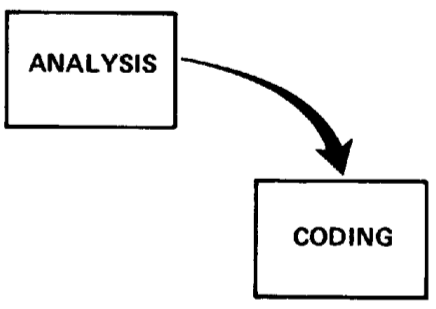
\includegraphics[width=.3\textwidth]{figures/small.png}
\alt<1>{%
\caption{Implementación de un programa pequeño de operaciones internas}
}{}
\end{figure}

\vspace{-1em}

\alt<2>{%
Un plan para hacer sistemas más grandes que se base en estos pasos está condenado al fracaso, ya que para estos se requiere muchos otros pasos de desarrollo para construir un software.
}{}

\end{frame}

\section{Bibliografía}

\begin{frame}[fragile]
\begin{thebibliography}{9}
\bibitem{royce70}
  \footnotesize
  Dr.\ Winston W.\ Royce \\
  \emph{Managing the Development of Large Software Systems} \\
  \texttt{IEEE Wescon},
  August 1970. \\
  \textit{Copyright ®1970 The Institute of Electrical and Electronics Engineers} \\
  {\scriptsize\url{https://cs.umd.edu/class/spring2003/cmsc838p/Process/waterfall.pdf}}
\end{thebibliography}
\end{frame}

\end{document}
